\section{Programmierung des ESP}
\label{mculogik}

Die Entwicklung eingebetteter Systeme erfordert eine präzise Abstimmung zwischen hardwarenahem Verhalten und übergeordneten Steuerungsprozessen. Insbesondere bei IoT-An\-wen\-dun\-gen, wie dem hier vorgestellten automatisierten Bewässerungssystem, kommt der softwareseitigen Ablaufsteuerung des Mikrocontrollers eine zentrale Rolle zu. 
\\
Die Funktionalität des Systems basiert auf dem koordinierten Zusammenspiel von Sensorik, drahtloser Netzwerkkommunikation, Aktorsteuerung und Datensynchronisation mit einem externen Backend.
\\
Der eingesetzte Mikrocontroller \texttt{ESP32-WROOM-32D} erweist sich aufgrund seiner integrierten WLAN-Funktionalität, Mehrkernarchitektur und Echtzeitfähigkeit als besonders geeignet für diese Anwendung. 
\\
Zudem bietet das zugrunde liegende ESP-IDF-Framework eine modulare und hardwarenahe Entwicklungsumgebung, die eine präzise Steuerung und effiziente Ressourcenverwaltung ermöglicht.
\\
Dieses Kapitel behandelt die programmtechnische Umsetzung der Systemlogik auf dem verwendeten Mikrocontroller (ESP32-WROOM-32D), wobei die eingesetzte Softwarearchitektur auf dem ESP-IDF-Framework basiert. Der Fokus liegt auf der Initialisierungslogik, der zyklischen Erfassung und Verarbeitung von Sensordaten, der Steuerung der Pumpe sowie der Einbindung in eine gesicherte MQTT-Kommunikationsstruktur. Die Interaktion mit dem Benutzer erfolgt sowohl über ein lokales Webinterface als auch über hardwareseitige Bedienelemente. 
\\
Insgesamt lässt sich die Entwicklung in zwei Teilbereiche unterteilen: Die Initialisierung des Mikrocontrollers und der laufende Betrieb. Diese beiden Bereiche sind eng miteinander verknüpft, da die Initialisierung die Grundlage für alle nachfolgenden Prozesse bildet.
\\
Ziel dieses Kapitels ist es, die internen Abläufe des Mikrocontrollers in strukturierter Form darzustellen, um sowohl die logische Abfolge als auch die funktionalen Abhängigkeiten nachvollziehbar zu machen. Die beiden Teilbereiche werden jeweils in ihrem eigenen Kapitel genauer betrachtet. Dazu wird zunächst ein abstrahierter Ablaufplan vorgestellt, welcher die zentralen Prozessschritte visuell abbildet. Dabei stellt ein je ein Eingefärbter bereich ein Funktion dar, welche durch das erste Element des Bereichs angegeben wird. Die darauffolgenden Elemente werden innerhald dieser Funktion ausgeführt. 
\\
Im Anschluss erfolgt eine schrittweise Low-Level-Beschreibung der internen Ablauflogik auf Basis des realisierten Programmcodes.
\\
\subsection{Initialisierung des ESP}
\label{sec:initlogik}

Die Initialisierungslogik des Mikrocontrollers stellt den operativen Ausgangspunkt für den gesamten Lebenszyklus des automatisierten Bewässerungssystems dar. Unmittelbar nach dem Systemstart des ESP32 übernimmt sie die Aufgabe, einen konsistenten und vollständig betriebsfähigen Ausgangszustand herzustellen. Dazu gehört insbesondere die Inbetriebnahme der netzwerkbasierten Kommunikationsschnittstellen, die Einbindung in den Authentifizierungsprozess mit dem Backend, die Bereitstellung eines Benutzerinterfaces zur Konfiguration sowie die Initialisierung interner Systemdaten.
\\
Die Initialisierung ist in der Funktion \texttt{device\_init()} im Modul \texttt{device\_manager.c} implementiert und wird aus dem zentralen Einstiegspunkt \texttt{app\_main()} in \texttt{main.c} aufgerufen. Erst wenn alle Voraussetzungen – insbesondere eine erfolgreiche WLAN-Verbindung und eine gültige Registrierung am Backend – erfüllt sind, gilt die Initialisierungsphase als abgeschlossen. Der Status wird über die Funktion \texttt{device\_init\_done()} überwacht, sodass nachfolgende Systemkomponenten (z.\,B. Sensorik, Zeitsynchronisation, MQTT-Kommunikation) erst im vollständig initialisierten Zustand gestartet werden.
\\
Darüber hinaus umfasst die Initialisierung eine robuste Reset-Funktionalität, die es ermöglicht, den Mikrocontroller über einen dedizierten GPIO-Pin manuell auf Werkseinstellungen zurückzusetzen. Eine zeitsensitive Tasterauswertung mit visueller Rückmeldung über die Status-LED garantiert dabei die absichtliche Auslösung. Zusätzlich ist die gesamte Netzwerkinitialisierung fehlertolerant gestaltet: Sollte ein Verbindungsversuch zur hinterlegten WLAN-Infrastruktur wiederholt fehlschlagen, wechselt das System automatisch in den Konfigurationsmodus (SoftAP) und stellt dem Benutzer ein lokales Webinterface zur Verfügung. Auf diese Weise wird eine autonome Wiederherstellung der Konnektivität ohne externe Eingriffe ermöglicht.

\begin{figure}[H]
	\centering
	\vspace{0pt} % verhindert Abstand oben
	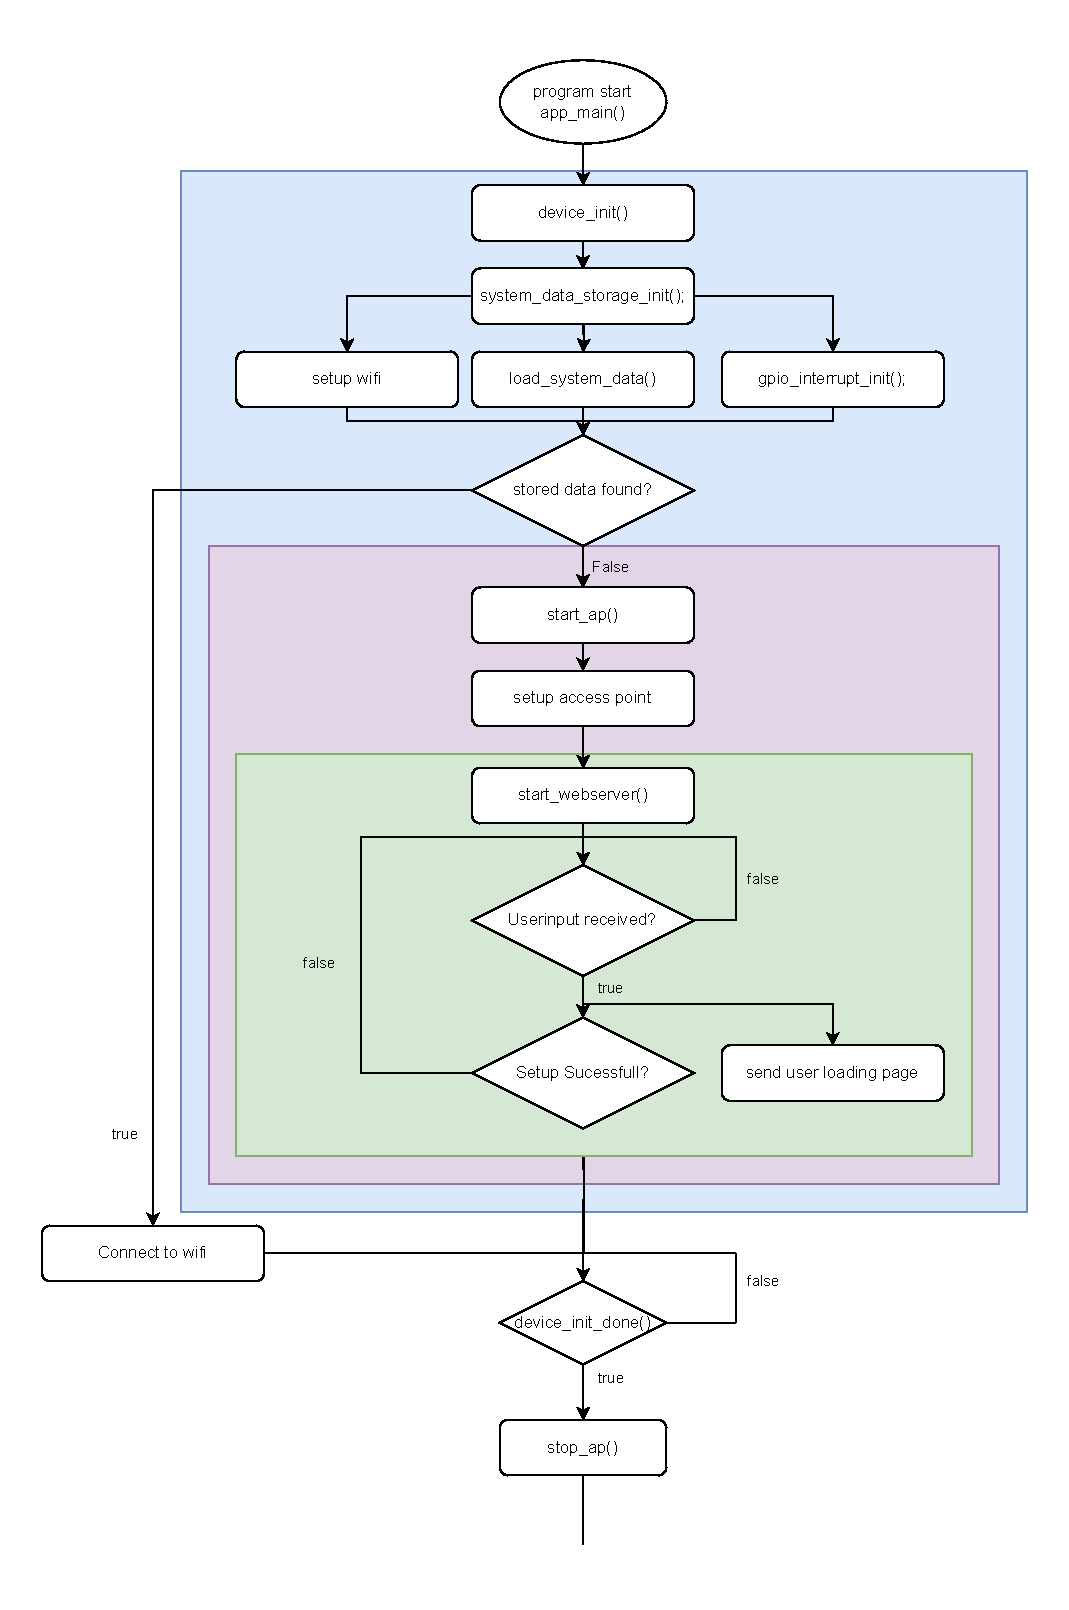
\includegraphics[width=1.1\textwidth, height=0.95\textheight, keepaspectratio]{./img/ESP_PAP.drawio.pdf}
	\caption{Ablaufplan Initialisierung des ESP}
	\label{fig:pap_esp32}
\end{figure}
\newpage

\subsubsection{Initialisierung des persistenten Speichers (NVS):}  
Der erste Schritt der Initialisierung besteht in der Aktivierung des nichtflüchtigen Speichers. Hierbei wird der sogenannte Non-Volatile Storage (NVS) über die Funktion \texttt{\url{nvs\_flash\_init()}} initialisiert. Dieser dient als zentrale, dauerhaft verfügbare Speicherstruktur zur Ablage von Konfigurationsdaten wie WLAN-Zugang, Authentifizierungstoken oder Zielwerten der Sensorik. Sollte der Speicher beschädigt sein oder durch ein Versionsupdate inkonsistent geworden sein, wird dies über die Rückgabecodes
\\
\texttt{ESP\_ERR\_NVS\_NO\_FREE\_PAGES} oder \texttt{ESP\_ERR\_NVS\_NEW\_VERSION\_FOUND} erkannt. 
\\
In diesem Fall wird über \texttt{nvs\_flash\_erase()} ein vollständiger Reset des Speichers durchgeführt. Die Architektur ist damit gegen veraltete oder inkonsistente Daten abgesichert und stellt eine fehlerfreie Persistenzlogik sicher.

\subsubsection{Laden und Strukturierung der Systemdaten:}  
Nach erfolgreicher NVS-Initialisierung wird über \texttt{load\_system\_data()} versucht, die Konfigurationsstruktur \texttt{system\_data\_t} aus dem Speicher zu laden. Diese Struktur enthält die meisten betriebskritischen Parameter, darunter:
\begin{itemize}
	\item Sensora-Nutzername,
	\item MQTT-Zugangsdaten (Benutzername, Passwort, Topics),
	\item Controller-Identifikation (ID, Modell),
	\item Sensor-Zielwerte (z.\,B. Bodenfeuchte, Temperatur, Luftfeuchte, Licht),
	\item Token für die Authentifizierung (Hardware und Software),
	\item Registrierungsstatus.
\end{itemize}
Ist der Speicherzugriff erfolgreich und die Daten konsistent, werden sie in einer lokalen Instanz gespeichert und stehenso für weitere verwendung zur Verfügung. Andernfalls verbleibt das System im Zustand \enquote{unregistriert} und leitet automatisch in den Setup-Modus über. 
\\
Zusätlich wird versucht die WLAN-Daten aus dem NVS zu laden. Diese sind werden allerdings direkt vom \texttt{esp\_wifi} Modul verwaltet und sind daher nicht Bestandteil der \texttt{system\_data\_t}-Struktur. Die WLAN-Daten werden über die Funktion \texttt{esp\_wifi\_get\_config()} geladen und in einer lokalen Instanz gespeichert. Diese Daten sind für die Registrierung des Geräts am Backend erforderlich und werden im weiteren Verlauf benötigt. Sind sie nicht vorhanden so wird das System ebenfalls in den Setup-Modus versetzt.

\subsubsection{Initialisierung der Status-LED:}  
Die Status-LED dient als primäres Feedbackinstrument für den Benutzer. Die LED ist über GPIO 2 angebunden und wird über das Modul \texttt{led\_control.c} gesteuert. Nach \texttt{led\_init()} ist der Pin als Ausgang initialisiert und standardmäßig deaktiviert. Die Logik unterscheidet mehrere Zustände:
\begin{itemize}
	\item \texttt{led\_blink\_start()}: SoftAP-Modus aktiv,
	\item \texttt{led\_on()}: System betriebsbereit und registriert,
	\item \texttt{led\_off()}: Fehlerzustand oder Resetphase.
\end{itemize}
Die Blinklogik ist als separate FreeRTOS-Task realisiert und damit unabhängig vom Hauptprogrammzyklus ausführbar, was insbesondere für Interrupt-gesteuerte Prozesse wie den Reset-Button entscheidend ist.
\\
Die aufruf der \texttt{led\_init()} erfolgt direkt nach der NVS-Initialisierung innerhalb der \texttt{device\_init()}. Dies stellt sicher, dass die LED-Logik auch bei einem Reset des NVS sofort verfügbar ist. 
\subsubsection{Einrichtung des Hardware-Resets via GPIO:}  
Um einen vollständigen Werksreset zu ermöglichen, wurde GPIO 0 als Eingangsquelle mit Pull-Up-Widerstand und fallender Flanke konfiguriert. Wird der Taster gedrückt, löst die Interrupt-Service-Routine \texttt{gpio\_isr\_handler()} eine Notification aus, die an die Task \texttt{reset\_task()} übergeben wird. Diese prüft, ob der Taster mindestens fünf Sekunden lang gedrückt bleibt. Während der Haltezeit blinkt die LED, um visuelles Feedback zu geben. Wird die Haltezeit überschritten, erfolgt:
\begin{enumerate}
	\item Stoppen des Wi-Fi-Treibers,
	\item Zurücksetzen der WLAN-Konfiguration (\texttt{esp\_wifi\_restore()}),
	\item Löschen aller Systemdaten aus dem NVS (\texttt{erase\_system\_data()}),
	\item Neustart des Controllers (\texttt{esp\_restart()}).
\end{enumerate}
Diese robuste, mehrstufige Logik verhindert unbeabsichtigte Rücksetzungen und garantiert eine sichere Wiederherstellung des Auslieferungszustands.

\subsubsection{Netzwerkstack und Eventsystem:}  
Die nächsten Initialisierungsschritte betreffen die Netzwerkkommunikation. Über \texttt{\url{esp\_netif\_init()}} wird die TCP/IP-Stack-Grundstruktur geladen. Anschließend wird ein zentraler Event-Loop mit \texttt{esp\_event\_loop\_create\_default()} erstellt, der später für alle netzwerkbezogenen Ereignisse zuständig ist. Zwei Interfaces werden parallel konfiguriert:
\begin{itemize}
	\item \texttt{esp\_netif\_create\_default\_wifi\_sta()} für den Station-Modus,
	\item \texttt{esp\_netif\_create\_default\_wifi\_ap()} für den SoftAP-Modus.
\end{itemize}
Durch die parallele Konfiguration kann der Controller sowohl als Client im Heimnetzwerk als auch als Access Point zur Erstkonfiguration agieren.

\subsubsection{Wi-Fi-Initialisierung und Event-Handler:}  
Das Wi-Fi-Modul wird über \texttt{esp\_wifi\_init()} mit einer Default-Konfiguration aktiviert. Die Registrierung von Event-Handlern erfolgt für zwei Eventtypen:
\begin{itemize}
	\item \texttt{WIFI\_EVENT}: Reaktion auf Verbindungsstart, -abbruch und Authentifizierungsfehler.
	\item \texttt{IP\_EVENT\_STA\_GOT\_IP}: Signalisiert erfolgreiche IP-Vergabe im Station-Modus.
\end{itemize}
Sobald eine Verbindung hergestellt ist und eine IP-Adresse bezogen wurde, wird der Status in der LED reflektiert. Bei mehrfachen Verbindungsabbrüchen (>5) wird automatisch in den AP-Modus zurückgeschaltet, um einen Konfigurationsfehler beheben zu können.

\subsubsection{Entscheidung über den Betriebsmodus (STA vs. SoftAP):}  
Die Entscheidung, ob das Gerät im Betriebsmodus (WLAN-Client) oder Setup-Modus (Access Point) starten soll, basiert auf den geladenen Systemdaten. Sind sowohl WLAN-Zugangsdaten als auch ein positiver Registrierungsstatus im NVS gespeichert, erfolgt der Start im STA-Modus. Der Controller versucht über \texttt{esp\_wifi\_set\_mode(WIFI\_MODE\_STA)} und \texttt{esp\_wifi\_start()} eine Verbindung aufzubauen. Andernfalls startet das System im SoftAP-Modus über \texttt{start\_ap()}.

\subsubsection{SoftAP-Modus und Webserver zur Konfiguration:}  
Im Setup-Modus stellt das System einen offenen WLAN-Access-Point mit dem Namen \enquote{Sensora} bereit. Parallel dazu wird ein HTTP-Webserver gestartet, der ein in \texttt{\url{wifi\_setup\_html.h}} eingebettetes Formular zur Verfügung stellt. Hier können SSID, Passwort und Benutzername eingegeben werden. Nach der Formulareinsendung wird über \texttt{esp\_wifi\_set\_config()} die neue Konfiguration übernommen und ein Verbindungsversuch gestartet. Eine JavaScript-basierte Statusabfrage im Browser informiert über Fortschritt und Fehlerzustände (z.\,B. keine Verbindung oder Backend nicht erreichbar). Die Benutzereingaben werden in der Systemstruktur gespeichert und sind ab diesem Moment Bestandteil der persistierten Konfiguration.

\subsubsection{Geräteregistrierung über den Authentifizierungsdienst:}  
Nach erfolgreichem Verbindungsaufbau über die im Webinterface eingegebenen WLAN-Daten wird die Registrierung des Geräts ausgelöst. Diese erfolgt über die Funktion \texttt{\url{register\_device()}} im Modul \texttt{auth\_service.c}. Ziel des Prozesses ist es, den Controller eindeutig beim zentralen Authentifizierungsserver zu identifizieren und verschlüsselte Zugangsdaten für den MQTT-Broker zu erhalten. Die Logik basiert auf einem mehrstufigen Challenge-Response-Verfahren mit HMAC-gesicherter Kommunikation und symmetrischer Fernet-Verschlüsselung (basierend auf AES-128 im CBC-Modus).

Die Registrierung umfasst folgende Schritte:
\begin{enumerate}
	\item Erstellung eines HMAC-basierten Token-Hashes aus Hardware- und Software-Token.
	\item Senden des Hashes zusammen mit dem Benutzernamen an die API \texttt{\url{/api/controller/init}}.
	\item Empfang einer zufälligen Challenge vom Server (Base64-codiert).
	\item Berechnung einer HMAC-Response auf Basis der Challenge und des Hardware-Tokens.
	\item Antwort über die API \texttt{/api/controller/verify}, zusammen mit dem ursprünglichen Token-Hash.
	\item Erhalt eines Fernet-codierten Credential-Tokens, das folgende Informationen enthält:
	\begin{itemize}
		\item MQTT-Benutzername und Passwort,
		\item Controller-ID und Modell,
		\item Publish- und Subscribe-Topics,
		\item Broker-URL, Port und SSL-Informationen.
	\end{itemize}
\end{enumerate}

\noindent Zur Validierung der Authentizität des Tokens sendet der Server zusätzlich einen sogenannten \texttt{credential\_key}, der lokal gegen einen HMAC-Vergleichswert verifiziert wird. Erst wenn diese Validierung erfolgreich ist, beginnt die Entschlüsselung des Tokens.

\subsubsection{Manuelle Implementierung der Fernet-Entschlüsselung:}  
Da im ESP32/ESP-IDF-Ökosystem keine native Unterstützung für Fernet besteht, wurde die gesamte Entschlüsselungslogik auf Byte-Ebene manuell umgesetzt. Diese umfasst:
\begin{itemize}
	\item Umwandlung von URL-safe Base64 in reguläres Base64 (inkl. Padding-Korrektur),
	\item Decodierung des Tokens mit \texttt{mbedtls\_base64\_decode()},
	\item Extraktion von Version, Timestamp, IV, Ciphertext und HMAC aus dem dekodierten Token,
	\item HMAC-Validierung des Tokens mit dem empfangenen Schlüssel zur Integritätsprüfung,
	\item Entschlüsselung des Payloads mit AES-128 im CBC-Modus über \texttt{\url{mbedtls\_aes\_crypt\_cbc()}},
	\item Entfernung und Validierung des PKCS\#7-Paddings.
\end{itemize}

Diese Implementierung stellte hohe Anforderungen an Genauigkeit im Umgang mit Speicherpuffern, Byte-Reihenfolgen und Formatierungsvorgaben. Zur Validierung wurden sämtliche Zwischenstände gegen Python-Referenzwerte getestet. Fehler in Padding-Handling oder IV-Länge führten während der Entwicklung regelmäßig zu Speicherverletzungen oder inkorrekten Dekodierungen. Dadurch wurde die Notwendigkeit einer präzisen und robusten Implementierung deutlich. Die gesamte Logik ist in der Funktion \texttt{decrypt\_fernet\_token()} im Modul \texttt{auth\_service.c} zusammengefasst.

\subsubsection{Speicherung und Abschluss der Registrierung:}  
Nach erfolgreicher Entschlüsselung werden alle empfangenen Felder aus dem Credential-Payload in die Struktur \texttt{system\_data\_t} überführt. Zusätzlich wird der Registrierungsstatus auf \texttt{true} gesetzt. Der gesamte Datenblock wird abschließend über \texttt{save\_system\_data()} dauerhaft im Flash gespeichert. Temporäre Speicherbereiche für MQTT-Daten und URLs werden aus dem Heap freigegeben. Dieser Mechanismus sichert sowohl Speicherstabilität als auch Datenintegrität und bildet die Basis für alle folgenden Kommunikationsprozesse.

\subsubsection{Abschluss der Initialisierung durch Deaktivierung des Setup-Modus:}  
Sobald Registrierung und Netzwerkverbindung erfolgreich abgeschlossen sind, endet eine while Schleife in \texttt{app\_main()}, da die Funktion \texttt{device\_init\_done} nun true returned. Danach wird der Setup-Modus beendet. Hierzu erfolgt im Hauptprogramm \texttt{app\_main()} ein expliziter Aufruf von \texttt{stop\_ap()}. Diese Funktion schaltet den Access Point ab, stoppt den HTTP-Webserver und wechselt den Betriebsmodus von \texttt{WIFI\_MODE\_APSTA} nach \texttt{WIFI\_MODE\_STA}. Dabei wird sichergestellt, dass keine Verbindungsversuche mehr mit dem offenen Netzwerk erfolgen und alle Schnittstellen auf eine abgesicherte Betriebsumgebung migriert werden.
\\
Ein typischer Ablauf von \texttt{stop\_ap()} umfasst:
\begin{enumerate}
	\item Überprüfung des aktuellen Betriebsmodus,
	\item Abschaltung des Webservers mit \texttt{httpd\_stop()},
	\item Wechsel in den reinen STA-Modus mittels \texttt{esp\_wifi\_set\_mode()},
	\item Soft-Restart des Wi-Fi-Treibers zur Sicherstellung eines sauberen Zustands,
	\item Reconnect-Versuch zur bekannten SSID bei verlorener Verbindung (optional),
	\item LED-Signalisierung durch Stoppen des Blinkens und dauerhaftes Einschalten.
\end{enumerate}

\noindent Diese Umstellung ist notwendig, da der SoftAP-Modus als temporäres Konfigurationsmittel konzipiert ist und im Normalbetrieb ein Sicherheitsrisiko darstellen würde.

\subsubsection{Abschlussprüfung der Initialisierung:}  
Nach Durchführung aller Schritte verbleibt das System im verbundenen, registrierten Zustand und ist bereit zur Ausführung der nachgelagerten Subsysteme. Der Status wird über die Funktion \texttt{device\_init\_done()} regelmäßig geprüft. Diese liefert den Wert \texttt{true}, sobald sowohl eine gültige IP-Adresse bezogen wurde (\texttt{is\_sta\_connected()}) als auch der \texttt{registered}-Status in \texttt{system\_data\_t} auf \texttt{true} gesetzt ist.

Erst wenn diese Bedingung erfüllt ist, werden in \texttt{app\_main()} die weiteren Initialisierungen durchgeführt:
\begin{itemize}
	\item Zeitsynchronisation mit SNTP über \texttt{initialize\_sntp()} und \texttt{wait\_for\_time\_sync()},
	\item Initialisierung der MQTT-Verbindung über \texttt{solace\_init()},
	\item Start der Sensorik und Bewässerungslogik.
\end{itemize}

\noindent Der Initialisierungsprozess ist damit abgeschlossen. Das System befindet sich fortan im überwachten Betriebsmodus und kann vollständig autonom auf externe Kon
